\documentclass[12pt,a4paper]{article}
\usepackage[utf8]{inputenc}
\usepackage[german]{babel}
\usepackage[T1]{fontenc}
\usepackage{times}
\usepackage{graphicx}
\usepackage{url}
\usepackage{color}
\usepackage{setspace}
\usepackage{enumerate}
\usepackage{amsmath}
\usepackage{amsfonts}
\usepackage{amssymb}
\usepackage{subfigure}
\usepackage{float}
\usepackage{stix}
\title{Kombinatorik}
\author{Henrik Tscherny}
\begin{document}
\maketitle
\tableofcontents

\section{Graphen}
\textbf{Notation/Definition}\\
\begin{itemize}
\item Menge aller k-elementigen Teilmengen von S: $\binom{S}{k}$\\
es gilt: $\bigl | \binom{S}{k} \bigl | \, = \, \binom{\vert S \vert}{k}$
\item Graph: $G \,=\, (V,E)$
\item komplementärer Graph: $\bar{G} \, = \, (V, \binom{V}{2} \setminus E)$\\
es gilt: $\bar{\bar{G}} = G$ (tausche Kanten mit nicht-Kanten)
\item Knotenmenge: $V(G)$
\item Kantenmenge: $E(G) \subseteq \binom{V}{2}$
\item Nachbarschaft: $N(s) = \{n \in V(G) \,\vert\, \{n,s\} \in  E(G),\, s\in S\subseteq V(G) \}$
\item Grad von v in G: $deg_G(v) = |N(v)|$
\item k-regulärer G: $\forall v\in V(G): deg_G(v) = k$ (Jeder Knoten hat den Grad k)
\item Graphen-Isomorphie: $f: V(G) \rightarrow V(H)$ mit\\
$\{u,v\} \in E(G) \Leftrightarrow \{f(u),f(v)\} \in E(H)$ und f Bijektion
\item Subgraph: $V(H) \subseteq V(G), \: E(H) \subseteq E(G) \cap \binom{V(H)}{2}$\\
$\cap \binom{V(H)}{2}$ = keine neuen Kanten (solche nicht in G) erlaubt
\item induzierter Subgraph: Enthält der Subgraph H einen Knoten auf G so enthält H auch alle mit diesem Knoten in Verbindung stehenden Kanten aus G, sofern der jeweilige Partnerknoten ebenfalls in H liegt\\
$E(H) = E(G) \cap \binom{V(H)}{2}$\\
man schreibt $G[V]$ für den Subgraph G induziert durch die Knotenmenge V\\
Sei $G-x$ der Subgraph von G induziert durch $V(G)\setminus\{x\}$
\item Walk: Weg von einem Knoten zu einem anderen\\
offen: Startpunkt $\neq$ Endpunkt, geschlossen: Startpunkt = Endpunkt
\item Pfad: Ein weg ohne Schleifen mit der Länge 1
\item Verbundener Graph: Es ex. ein Walk von jeden jedem zu jedem Knoten\\
\textbf{Ein Graph G ist verbunden gdw. er nicht als disjunkte Vereinigung von zwei nicht-leeren Teilgraphen erzeugt werden kann}
\item k-verbundener Graph: Es existiert für alle $a,b \in V$ k paarweise unabhängige Pfade von a nach b
\end{itemize}
\begin{figure}[H]
\subfigure[Graph]{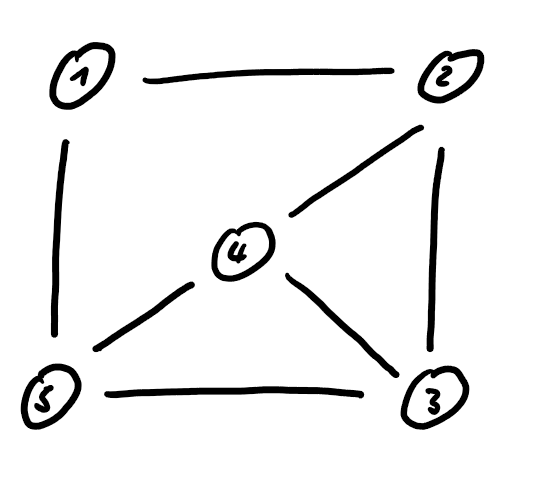
\includegraphics[width=.22\textwidth]{./resources/graph1.png}}
\subfigure[Subgraph]{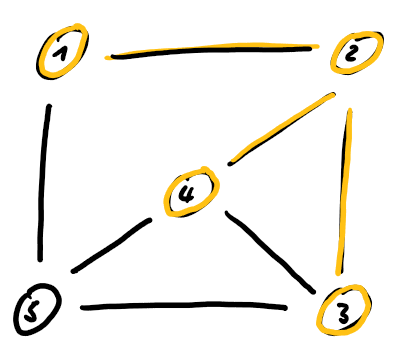
\includegraphics[width=.22\textwidth]{./resources/subgraph1.png}}
\subfigure[ind. Subgraph]{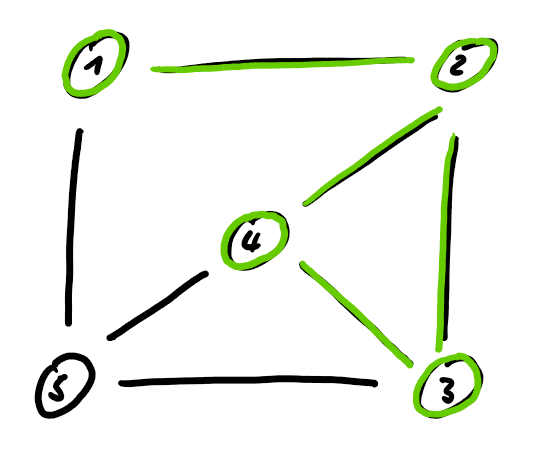
\includegraphics[width=.23\textwidth]{./resources/ind_subgraph1.png}}
\subfigure[kein Subgraph]{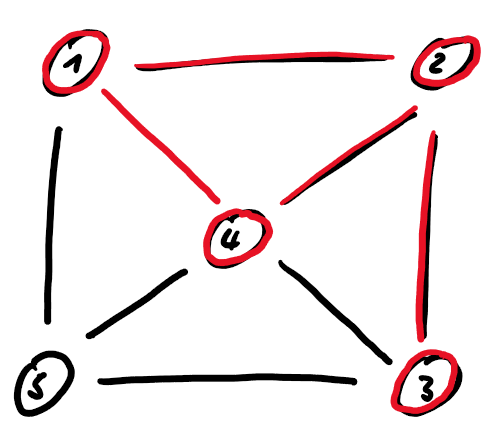
\includegraphics[width=.23\textwidth]{./resources/no_subgraph1.png}}
\end{figure}
\textbf{Spezielle Graphen}
\begin{itemize}
\item \textbf{Clique (vollst. Graph)}: $K_n = G = (V,E)$ mit\\
$ V := \{1,...,n\}, \, E = \binom{V}{2}$\\
es gilt: $\bar{K_n} = I_n$
\item \textbf{Unabhängiger Graph}: $I_n = G = (V,E)$ mit $V = \{1,...,n \} \, E = \emptyset$\\
es gilt: $\bar{I_n} = K_n$
\item \textbf{Graph mit Pfad der Länge n}: $P_n = G = (V, E)$ mit  $V = \{1,...,n \} \, E = \{\{1, 2\},\{2, 3\}, \{n-1, n\}\}$
\item \textbf{Graph mit Kreis der Länge n} $C_n = G = (V, E)$ mit $V = \{1,...,n-1 \} \, E = \{\{i, j\} \vert (i-j) \equiv 1\, (mod\, n) \}$ (n Knoten und n Kanten)

\end{itemize}
\begin{figure}[H]
\subfigure[$K_5$]{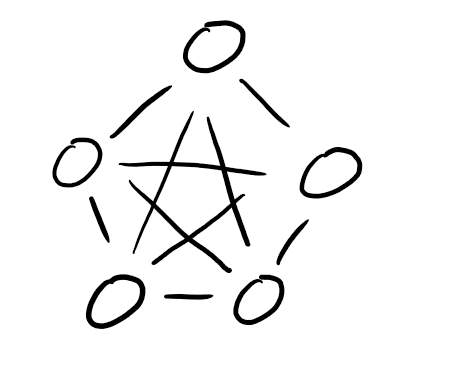
\includegraphics[width=.225\textwidth]{./resources/k5.png}}
\subfigure[$I_5$]{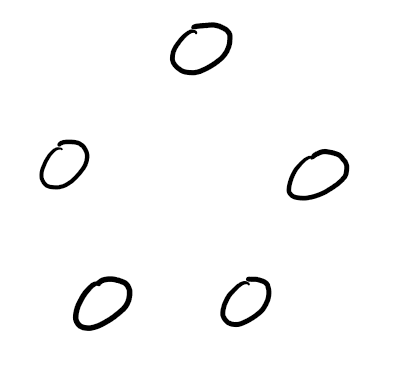
\includegraphics[width=.225\textwidth]{./resources/i5.png}}
\subfigure[$P_5$]{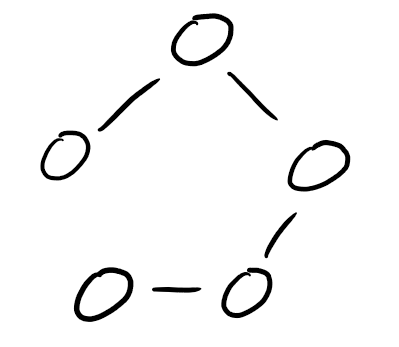
\includegraphics[width=.225\textwidth]{./resources/p5.png}}
\subfigure[$C_5$]{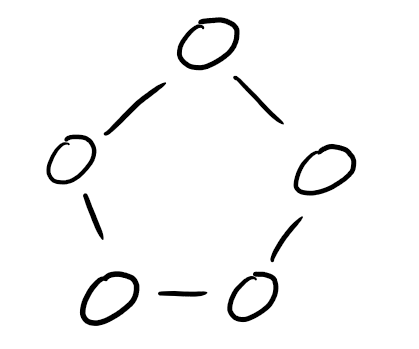
\includegraphics[width=.225\textwidth]{./resources/c5.png}}
\end{figure}

\textbf{Färbbarkeit}\\
\begin{itemize}
\item k-Färbbarkeit: $f: V(G) \rightarrow \{0,...,k-1 \}$, sodass\\
$f(u) \neq f(v) \: \forall \{u,v\} \in E(g)$\\
direkt miteinander Verbundene Knoten haben unterschiedliche Farben
\item \textbf{Lemma}: Jeder endliche Graph G ist bipartit gdw. er keine Kreise ungerader Länge enthält
\end{itemize}

\textbf{Bäume}
\begin{itemize}
\item Ein Graph ohne Kreise ist ein Wald
\item Ein Verbundener Graph ohne Kreise ist ein Baum
\item Ein Wald ist eine disjunkte Vereinigung von Bäumen
\item Jeder Baum ist bipartit
\item Folgende Definitionen sind Äquivalent:
\begin{itemize}
\item G ist ein Baum
\item $\vert E \vert = \vert V \vert -1$
\item $\vert E \vert \leq \vert V \vert -1 $
\item G hat maximal viele Kanten ohne Kreise zu enthalten
\item G hat minimal viele Kanten und ist zusammenhängend
\item für alle Knoten in G existiert paarweise ein eindeutiger Pfad
\end{itemize}
\end{itemize}

\subsection{Matchings}
\textbf{Definitionen}\\
\begin{itemize}
\item Ein Matching ist eine Teilmenge der Kantenmenge von G, sodass diese \textbf{paarweise disjunkt} sind, d.h. jeder nur max. einen Partner hat ($\forall u, v \in M: \, u \cap v = \emptyset$)
\item gilt $2 \vert M \vert = \vert V \vert$, d.h. es gibt doppelt so viele Knoten wie Kanten in M (jeder hat genau einen Partner, d.h. jeder Knoten wurde gematched), dann ist es ein \textbf{perfektes Matching}
\item \textbf{für jeden bipartiten k-regulären Graphen} mit $k \geq 1$ gibt es ein \textbf{perfektes Matching}
\item für $\{x,y\} \in M$ heißt y der \textbf{Partner} von x
\item Sei S $\subseteq V(G)$, dann ist M ein Matching in S wenn für jedes $s\in S$, s in M vorkommt, d.h. jeder Knoten aus S kommt in einer Kante von M vor
\item Ein Pfad bzgl. M heißt \textbf{alternierend}, wenn er abwechselnd Kanten über $E(G) \setminus M$ und M verläuft
\item Ein alternierender Pfad heißt \textbf{augmentierend} wenn Start und Endpunkt keinen Partner in M haben
\end{itemize}
\begin{figure}[H]
\centering
\subfigure[ein mögl. M auf G]{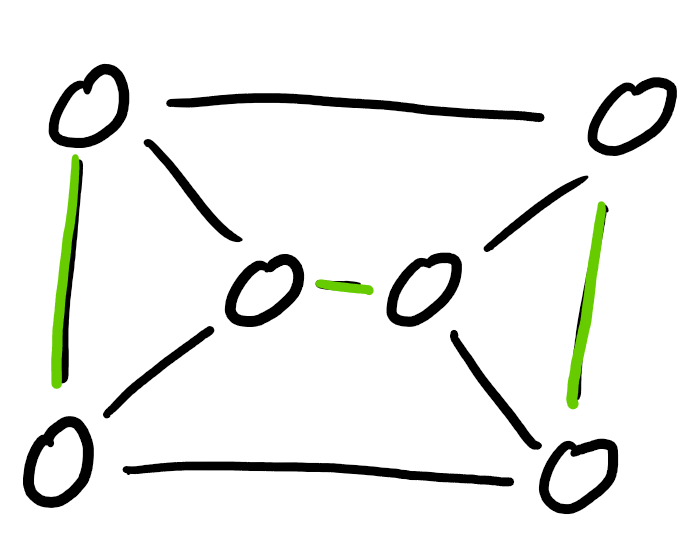
\includegraphics[width=.23\textwidth]{./resources/matching.png}}
\subfigure[alternierender Pfad]{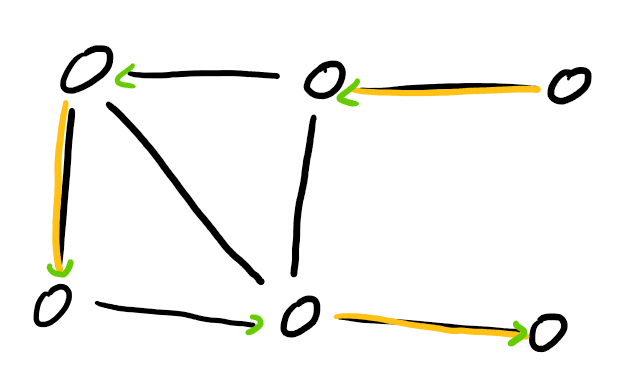
\includegraphics[width=.3\textwidth]{./resources/alt_pfad.png}}
\subfigure[augmentierender Pfad]{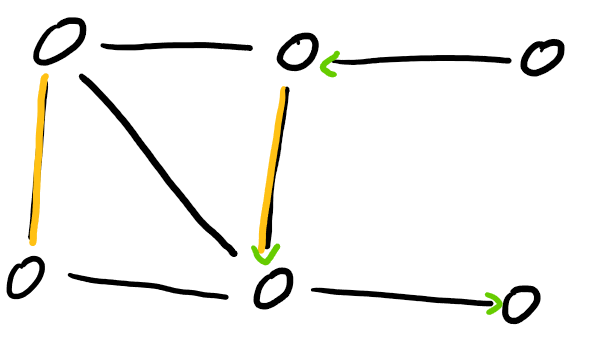
\includegraphics[width=.3\textwidth]{./resources/aug_pfad.png}}
\end{figure}

\paragraph{Lemma}
\flushleft
Sei P ein augmentierender Pfad und $M' = M \Delta P$, dann ist $M'$ wieder ein Matching und $\vert M' \vert > \vert M \vert$
\begin{figure}[H]
\centering
\subfigure[M in G mit augm. P]{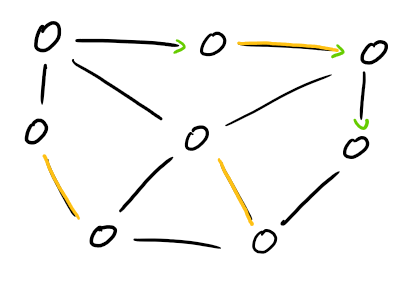
\includegraphics[width=.35\textwidth]{./resources/m1_graph.png}}
\subfigure[$P \Delta M$]{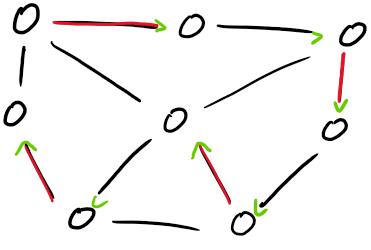
\includegraphics[width=.32\textwidth]{./resources/m2_graph.png}}
\end{figure}
\paragraph{Lemma von Berge}
\flushleft
Sei G ein endlicher Graph und M ein Matching in G. M ist \textbf{maximal} gdw. es \textbf{keine augmentieren Pfade in G bzgl. M gibt}

\textit{Beweis}:
\begin{itemize}
\item TODO
\end{itemize}


\paragraph{Heiratssatz}
\flushleft
Ein bipartiter Graph G hat ein Matching $A\subseteq V(G)$ gdw. $\forall S \subseteq A: \vert N(S) \vert \geq \vert S \vert$
\textbf{mögliche Darstellungen}:
\begin{itemize}
\item als Funktion
\begin{itemize}
\item Sei $A = (A_i)_{i\in I}$ eine Menge von endlichen Mengen
\item Gibt es eine \textit{injektive Auswahlfunktion} $\displaystyle f: I \rightarrow \bigcup_{i\in I} A_i$, sodass $\forall i \in I f(i) \in A_i$ gilt ?
\item Hall-Bedingung: $\displaystyle I_0 \subseteq I : \bigl\vert \bigcup_{i\in I_0} A_i \bigl\vert \geq \vert I_0 \vert$
\end{itemize}
\item als Realbeispiel
\begin{itemize}
\item Sei I eine Menge von Frauen
\item Sei X eine Menge von Männern, welche mit diesen Frauen befreundet sind
\item Lassen sich die Frauen mit den Männern so verheiraten, dass jede Frau einen befreundeten Mann heiratet
\item Note: Es gibt nur Monogame Beziehungen
\item Notwendige Bedingung: je k Frauen müssen mit mindestens k Männern befreundet sein (Hall-Bedingung)
\end{itemize}
\item Graphentheoretisch
\begin{itemize}
\item Sei G ein bipartiter Graph
\item Seien A, B Bipartionen von G, d.h. $A \cup B = G$ und $A \cap B = \emptyset$
\item Es gilt nun durch die Bipartitheit, dass jeder Nachbar eines Knotens aus A zu B gehört
\item Gibt es ein Matching in dem alle Knoten aus A vorkommen ?
\end{itemize}
\item aus dem Heiratssatz folgt ebenso:
\begin{itemize}
\item Sei F eine Menge an endlichen Teilmengen einer Menge X
\item F hat einen \textbf{Durchschnitt} gdw. F die Hall-Bedingung erfüllt
\item Beweis:
\begin{itemize}
\item TODO
\end{itemize}
\end{itemize}
\end{itemize}

\paragraph{Satz von König}
\flushleft
Sei G ein endlicher bipartiter Graph, dann ist die \textbf{Größe des größten Matchings} in G \textbf{gleich} der \textbf{minimalen Anzahl an Überdeckungen} in G\\

\textbf{Überdeckung}
\begin{itemize}
\item U ist eine Teilmenge der Knotenmenge V, wobei jede Kante aus G einen Knoten in G enthält
\item $U \subseteq V(G)$ mit $\forall e\in E(G) : e \in V(U)$
\item kurz: alle Knoten von G müssen mit U abgedeckt werden
\end{itemize}

\textbf{Beweis}
\begin{itemize}
\item TODO
\end{itemize}

\section{Dualität}
Die Essenz dualer Probleme liegt darin, dass immer gezeigt werden kann, dass sofern ein Sachverhalt gilt, ein dazu dualer Sachverhalt gilt und umgekehrt\\
\textbf{(P) $\Rightarrow$ $\lnot$ (D) und $\lnot$ (P) $\Rightarrow$ (D)}
\subsection{Dualität in der linearen Algebra}
Sei $A \in \mathbb{R}^{m\times n},\:x=(x_1,...,x_n)$ und $b \in \mathbb{R}^m$\\
Dann ist die Gleichung $Ax=b$ \textbf{unerfüllbar} gdw. das System\\
$(A\vert b)^{\top}y = (0,...,0,1)^\top$ \textbf{erfüllbar} ist 
\textbf{Beweis}
\begin{itemize}
\item ($\Leftarrow$)
\begin{itemize}
\item TODO
\end{itemize}
\item ($\Rightarrow$)
\begin{itemize}
\item TODO
\end{itemize}
\end{itemize}

\subsection{gewichtete Matchings}
Sei $G=(V,E)$ ein Graph wobei $\forall e\in E(G)$ zusätzlich ein Gewicht $w_e \in \mathbb{R}$ festgelegt wird\\
Das \textbf{Gewicht eines Matchings} ist dann $\displaystyle w(M) := \sum_{e\in M} w_e$

\textbf{Suche nach einem Matching mit maximalem Gewicht}\\
Dazu wird das Matchingproblem in G in ein LP umgeformt:
\begin{itemize}
\item $\forall e \in E(G) \, | \, x_e = \begin{cases} x_e = 0, & e \not\in M\\ x_e = 1, & e \in M \end{cases}$
\item $x_e$ gibt also an ob eine Kante e in G im Matching M liegt
\item Damit erhält man folgende \textbf{objective function}: $\displaystyle w(x) = \sum_{e\in M} w_e x_e$\\
$\rightarrow$ nur die Gewichte der ausgewählten Kanten ($x_e = 1$) werden summiert
\item \textbf{Nebenbedingung}: $\displaystyle w(M) = \sum_{\substack{e\in E(G)\\ v\in e}} x_1 = 1$\\
$\rightarrow$ jeder Knoten taucht nur in genau einer Kante in M auf
\end{itemize}

\subsection{Relaxation}

\end{document}